\chapter{Sprint 5 — Personalized Recommendations}

\section*{Introduction}
\addcontentsline{toc}{section}{Introduction}

Sprint 5 adds a \textbf{personalized recommendation engine} to the AR-API. The system learns
from each user's search queries, click events, and playlist additions, building a continuously
updated interest profile that drives a blended personalized and trending video feed. Three new
PostgreSQL tables and one Alembic migration extend the schema; the new module integrates
seamlessly with the existing FastAPI layered architecture.

%% ─── Sprint Backlog ─────────────────────────────────────────────────────────
\section{Sprint Backlog}

\begin{table}[H]
\centering
\caption{Sprint 5 Backlog}
\label{tab:sprint5_backlog_rec}
\begin{tabularx}{\textwidth}{clXcc}
\toprule
\textbf{ID} & \textbf{Story} & \textbf{Task} & \textbf{Effort (d)} & \textbf{Prio.} \\
\midrule
T6.1 & US-17 & Recommendation ORM models: search events, video events, interest profiles & 1   & M \\
T6.2 & US-17 & Alembic migration for recommendation tables                              & 0.5 & M \\
T6.3 & US-17 & Interest profile update on search/click event ingestion                 & 1   & M \\
T6.4 & US-17 & Weight-decay and boosting logic for category/tag/entity signals          & 0.5 & M \\
T6.5 & US-17 & Recommendation seed builder (recent events + profile aggregates)        & 1   & M \\
T6.6 & US-17 & Personalized + trending candidate retrieval via advanced-search         & 1   & M \\
T6.7 & US-17 & Blending pipeline: diversity cap, freshness bonus, exploration slice     & 1   & S \\
T6.8 & US-17 & \texttt{GET /recommendations} endpoint with limit and refresh params    & 0.5 & M \\
\bottomrule
\end{tabularx}
\end{table}

%% ─── Design ─────────────────────────────────────────────────────────────────
\section{Design}

\subsection{Use Case Diagram for Sprint 5}

Figure~\ref{fig:uc_sprint6} shows the actors and primary use cases for the recommendation
system. The \emph{Licensed User} drives the system through searches and video interactions,
while the \emph{Videos Search API} serves as an internal candidate provider.

\begin{figure}[H]
\centering
\begin{tikzpicture}[x=1cm, y=1cm]

%% ── Recommendation boundary ──────────────────────────────────────────────
\node[ucboundary, minimum width=8.4cm, minimum height=6.0cm,
      label={[font=\small\bfseries]above:Recommendation System}]
  (recbnd) at (4.2, -2.6) {};

\node[usecase] (uc_search_ev)  at (4.2, -1.0) {Record search event};
\node[usecase] (uc_click_ev)   at (4.2, -2.6) {Record click / view event};
\node[usecase] (uc_get_recs)   at (4.2, -4.2) {Get personalised feed};

%% ── User actor ───────────────────────────────────────────────────────────
\umlactor{-2.0}{-2.6}{Licensed\\User}

\draw[ucassoc] (-1.4,-2.1) -- (uc_search_ev.west);
\draw[ucassoc] (-1.4,-2.6) -- (uc_click_ev.west);
\draw[ucassoc] (-1.4,-3.1) -- (uc_get_recs.west);

%% ── Videos Search API actor ──────────────────────────────────────────────
\umlactor{11.0}{-4.2}{Videos\\Search API}

\draw[ucincl] (uc_get_recs.east) -- node[above, font=\fontsize{7}{8}\selectfont\itshape]
  {$\langle\langle$uses$\rangle\rangle$} (10.4,-4.2);

%% ── PostgreSQL actor ─────────────────────────────────────────────────────
\umlactor{11.0}{-1.0}{PostgreSQL}

\draw[ucincl] (uc_search_ev.east) -- node[above, font=\fontsize{7}{8}\selectfont\itshape]
  {$\langle\langle$persists$\rangle\rangle$} (10.4,-1.0);

\end{tikzpicture}
\caption{Sprint 5 use case diagram — Recommendation System}
\label{fig:uc_sprint6}
\end{figure}

\subsection{Recommendation Algorithm Overview}

The recommendation engine follows a three-stage pipeline shown in
Figure~\ref{fig:rec_pipeline}: \emph{signal ingestion}, \emph{seed construction}, and
\emph{candidate blending}.

\begin{figure}[H]
\centering
\begin{tikzpicture}[
  stage/.style={draw=teal!70!black, fill=teal!8, rounded corners=4pt,
    minimum width=3.6cm, minimum height=0.9cm,
    font=\small\bfseries, align=center},
  sub/.style={draw=gray!55, fill=gray!5, rounded corners=3pt,
    minimum width=3.2cm, minimum height=0.7cm,
    font=\fontsize{8}{9}\selectfont, align=center},
  arr/.style={->, >=Stealth, thick, teal!60!black},
  subarr/.style={->, >=Stealth, semithick, gray!60},
]
%% Stage 1
\node[stage] (s1) at (0, 0)     {1. Signal Ingestion};
\node[sub]   (s1a) at (-2.0,-1.3) {Search events\\(query + intent)};
\node[sub]   (s1b) at ( 2.0,-1.3) {Click/view events\\(video\_id + context)};

\draw[subarr] (s1a.north) -- (s1.south west);
\draw[subarr] (s1b.north) -- (s1.south east);

%% Stage 2
\node[stage] (s2) at (0, -3.0)  {2. Seed Construction};
\node[sub]   (s2a) at (-2.3,-4.3) {Profile weights\\(decay + top-k)};
\node[sub]   (s2b) at ( 2.3,-4.3) {Recent search events\\(last 30 queries)};

\draw[subarr] (s2a.north) -- (s2.south west);
\draw[subarr] (s2b.north) -- (s2.south east);

%% Stage 3
\node[stage] (s3) at (0, -6.0)  {3. Candidate Blending};
\node[sub]   (s3a) at (-2.3,-7.3) {Personalized\\candidates};
\node[sub]   (s3b) at ( 2.3,-7.3) {Trending\\candidates};

\draw[subarr] (s3a.north) -- (s3.south west);
\draw[subarr] (s3b.north) -- (s3.south east);

%% Stage connections
\draw[arr] (s1) -- node[right, font=\fontsize{8}{9}\selectfont]
  {update interest profile} (s2);
\draw[arr] (s2) -- node[right, font=\fontsize{8}{9}\selectfont]
  {categories + tags + entities} (s3);

%% Output
\node[stage, draw=blue!60!black, fill=blue!8] (out) at (0, -9.0) {Ranked Feed};
\draw[arr] (s3) -- node[right, font=\fontsize{8}{9}\selectfont]
  {diversity + freshness + exploration} (out);

\end{tikzpicture}
\caption{Three-stage recommendation pipeline}
\label{fig:rec_pipeline}
\end{figure}

\subsection{Sequence Diagrams}

\subsubsection{Search Event Ingestion}

Figure~\ref{fig:seq_rec_search} traces how a search event flows from the frontend to the
interest profile update. The profile is created on first event; subsequent events apply
exponential decay before boosting new signals.

\begin{figure}[H]
\centering
\begin{tikzpicture}[x=1cm, y=1cm, font=\fontsize{7}{8}\selectfont]
%% Participants
\node[sdFE]   (pPortal) at ( 0.0, 0) {Video Search\\Portal};
\node[sdBE]   (pAPI)    at ( 3.0, 0) {AR-API\\(recommendations)};
\node[sdData] (pDB)     at ( 6.5, 0) {PostgreSQL};

%% Lifelines
\foreach \x in {0.0, 3.0, 6.5}
  \draw[dashed, gray!50] (\x,-0.3) -- (\x,-10.2);

%% Messages
\draw[sdmsg] (0.0,-0.85) -- node[above, pos=0.5]{POST /recommendations/events/search \{query, parsed\_intent\}} (3.0,-0.85);
\draw[sdmsg] (3.0,-1.57) to[out=-30,in=30] node[right, pos=0.5]{validate payload (Pydantic)} (3.0,-2.29);

%% Insert event
\draw[sdmsg] (3.0,-3.01) -- node[above, pos=0.5]{INSERT user\_search\_events} (6.5,-3.01);
\draw[sdret] (6.5,-3.73) -- node[above, pos=0.5]{OK} (3.0,-3.73);

%% Get or create profile
\draw[sdmsg] (3.0,-4.45) -- node[above, pos=0.5]{SELECT user\_interest\_profiles WHERE user\_id=\$1} (6.5,-4.45);
\draw[sdret] (6.5,-5.17) -- node[above, pos=0.5]{profile row (or null $\rightarrow$ INSERT new)} (3.0,-5.17);

%% Apply decay + boost
\draw[sdmsg] (3.0,-5.89) to[out=-30,in=30] node[right, pos=0.5]{apply decay factor to all weights} (3.0,-6.61);
\draw[sdmsg] (3.0,-7.33) to[out=-30,in=30]
  node[right, pos=0.5]{boost category/tag/entity weights from parsed\_intent} (3.0,-8.05);

%% Flush
\draw[sdmsg] (3.0,-8.77) -- node[above, pos=0.5]{UPDATE user\_interest\_profiles (flush)} (6.5,-8.77);
\draw[sdret] (6.5,-9.49) -- node[above, pos=0.5]{200 OK \{saved: true\}} (3.0,-9.49);
\draw[sdret] (3.0,-9.49) -- (0.0,-9.49);

\end{tikzpicture}
\caption{Search event ingestion — interest profile update sequence}
\label{fig:seq_rec_search}
\end{figure}

\subsubsection{Click / View Event Ingestion}

Figure~\ref{fig:seq_rec_click} shows the click event path. Video-level context
(\texttt{categories}, \texttt{tags}, \texttt{entities}) is extracted from the request and
applied to the profile with higher weights than search signals.

\begin{figure}[H]
\centering
\begin{tikzpicture}[x=1cm, y=1cm, font=\fontsize{7}{8}\selectfont]
%% Participants
\node[sdFE]   (pPortal) at ( 0.0, 0) {Video Search\\Portal};
\node[sdBE]   (pAPI)    at ( 3.0, 0) {AR-API\\(recommendations)};
\node[sdData] (pDB)     at ( 6.5, 0) {PostgreSQL};

%% Lifelines
\foreach \x in {0.0, 3.0, 6.5}
  \draw[dashed, gray!50] (\x,-0.3) -- (\x,-10.2);

\draw[sdmsg] (0.0,-0.85) -- node[above, pos=0.5]{POST /recommendations/events/click \{video\_id, event\_type, event\_context\}} (3.0,-0.85);

\draw[sdmsg] (3.0,-1.57) -- node[above, pos=0.5]{INSERT user\_video\_events} (6.5,-1.57);
\draw[sdret] (6.5,-2.29) -- node[above, pos=0.5]{OK} (3.0,-2.29);

\draw[sdmsg] (3.0,-3.01) -- node[above, pos=0.5]{SELECT user\_interest\_profiles} (6.5,-3.01);
\draw[sdret] (6.5,-3.73) -- node[above, pos=0.5]{profile} (3.0,-3.73);

\draw[sdmsg] (3.0,-4.45) to[out=-30,in=30] node[right, pos=0.5]{apply decay} (3.0,-5.17);
\draw[sdmsg] (3.0,-5.89) to[out=-30,in=30]
  node[right, pos=0.5]{boost entity\_weights +2.5, category/tag from context} (3.0,-6.61);

\draw[sdmsg] (3.0,-7.33) -- node[above, pos=0.5]{UPDATE profile (flush)} (6.5,-7.33);
\draw[sdret] (6.5,-8.05) -- node[above, pos=0.5]{OK} (3.0,-8.05);
\draw[sdret] (3.0,-8.77) -- node[above, pos=0.5]{200 OK \{saved: true\}} (0.0,-8.77);

\end{tikzpicture}
\caption{Click/view event ingestion sequence}
\label{fig:seq_rec_click}
\end{figure}

\subsubsection{Personalized Recommendation Feed}

Figure~\ref{fig:seq_rec_feed} shows the full path for \texttt{GET /recommendations}. The AR-API
builds a seed from recent search events and the interest profile, queries the Videos Search API
twice (personalized and trending), blends and ranks candidates, and returns the final list.

\begin{figure}[H]
\centering
\begin{tikzpicture}[x=1cm, y=1cm, font=\fontsize{7}{8}\selectfont]
%% Participants
\node[sdFE]   (pPortal)  at ( 0.0, 0) {Portal};
\node[sdBE]   (pAPI)     at ( 2.5, 0) {AR-API};
\node[sdData] (pDB)      at ( 5.2, 0) {PostgreSQL};
\node[sdExt]  (pSearch)  at ( 8.5, 0) {Videos\\Search API};

%% Lifelines
\foreach \x in {0.0, 2.5, 5.2, 8.5}
  \draw[dashed, gray!50] (\x,-0.3) -- (\x,-18.5);

%% 1. Request
\draw[sdmsg] (0.0,-0.85) -- node[above, pos=0.5]{GET /recommendations?limit=12} (2.5,-0.85);

%% 2. Load profile
\draw[sdmsg] (2.5,-1.57) -- node[above, pos=0.5]{SELECT user\_interest\_profiles} (5.2,-1.57);
\draw[sdret] (5.2,-2.29) -- node[above, pos=0.5]{profile} (2.5,-2.29);

%% 3. Merge playlist signals
\draw[sdmsg] (2.5,-3.01) -- node[above, pos=0.5]{SELECT playlist video IDs} (5.2,-3.01);
\draw[sdret] (5.2,-3.73) -- node[above, pos=0.5]{video\_ids} (2.5,-3.73);
\draw[sdmsg] (2.5,-4.45) to[out=-30,in=30] node[right, pos=0.5]{merge into entity\_weights} (2.5,-5.17);

%% 4. Build seed from recent events
\draw[sdmsg] (2.5,-5.89) -- node[above, pos=0.5]{SELECT last 30 user\_search\_events} (5.2,-5.89);
\draw[sdret] (5.2,-6.61) -- node[above, pos=0.5]{events} (2.5,-6.61);
\draw[sdmsg] (2.5,-7.33) to[out=-30,in=30]
  node[right, pos=0.5]{aggregate categories/tags/entities from parsed\_intent} (2.5,-8.05);

%% 5. Merge seeds
\draw[sdmsg] (2.5,-8.77) to[out=-30,in=30]
  node[right, pos=0.5]{merge seeds (recent-first priority)} (2.5,-9.49);

%% 6. Personalized candidates
\draw[sdmsg] (2.5,-10.21) -- node[above, pos=0.5]{POST /api/videos/advanced-search \{query, categories, tags\}} (8.5,-10.21);
\draw[sdret] (8.5,-10.93) -- node[above, pos=0.5]{personalized candidates (3$\times$limit)} (2.5,-10.93);

%% 7. Trending candidates
\draw[sdmsg] (2.5,-11.65) -- node[above, pos=0.5]{POST /api/videos/advanced-search \{sort: views, desc\}} (8.5,-11.65);
\draw[sdret] (8.5,-12.37) -- node[above, pos=0.5]{trending candidates (2$\times$limit)} (2.5,-12.37);

%% 8. Load seen IDs
\draw[sdmsg] (2.5,-13.09) -- node[above, pos=0.5]{SELECT recent user\_video\_events + playlist videos} (5.2,-13.09);
\draw[sdret] (5.2,-13.81) -- node[above, pos=0.5]{seen video\_ids (last 200)} (2.5,-13.81);

%% 9. Blend
\draw[sdmsg] (2.5,-14.53) to[out=-30,in=30]
  node[right, pos=0.5]{blend 70\% personalized + 30\% trending; freshness, diversity, rotation, exploration} (2.5,-15.97);

%% 10. Return
\draw[sdret] (2.5,-16.69) -- node[above, pos=0.5]{200 OK \{items, total, seed, generated\_at\}} (0.0,-16.69);

\end{tikzpicture}
\caption{Personalized recommendation feed — full sequence diagram}
\label{fig:seq_rec_feed}
\end{figure}

%% ─── Implementation ────────────────────────────────────────────────────────
\section{Implementation}

\subsection{Recommendation Module}

The recommendation module (\texttt{app/recommendation/}) follows the standard AR-API layered
structure: \texttt{router.py} $\rightarrow$ \texttt{services.py} $\rightarrow$
\texttt{models.py} / \texttt{schemas.py}.

\subsubsection{API Endpoints}

\begin{table}[H]
\centering
\caption{Recommendation endpoints}
\label{tab:rec_endpoints}
\begin{tabularx}{\textwidth}{llX}
\toprule
\textbf{Method} & \textbf{Path} & \textbf{Description} \\
\midrule
POST & \texttt{/recommendations/events/search} &
  Ingest a search query + parsed intent; update the interest profile. \\
POST & \texttt{/recommendations/events/click} &
  Ingest a click/view event on a video; boost entity, category, and tag signals. \\
GET  & \texttt{/recommendations?limit=\&refresh=} &
  Return a blended personalized + trending video feed. \\
\bottomrule
\end{tabularx}
\end{table}

All three endpoints require a valid Clerk JWT (\texttt{Authorization: Bearer \ldots}) and
operate on the currently authenticated user's profile.

\subsubsection{Interest Profile and Weight Decay}

Each user has exactly one \texttt{user\_interest\_profiles} row (enforced by a
\texttt{UNIQUE} constraint on \texttt{user\_id}). The profile stores three \texttt{JSONB}
dictionaries: \texttt{category\_weights}, \texttt{tag\_weights}, and \texttt{entity\_weights}.
Keys are string signals (category names, tags, or video IDs); values are floating-point scores.

\paragraph{Update rule.}
On every incoming event, every existing weight is first multiplied by a decay factor
$\lambda = 0.97$ (configurable as \texttt{RECOMMENDATION\_DECAY\_FACTOR}), then the fixed
boost delta $\Delta$ for that signal is added:

\[
  w_k \leftarrow w_k \times \lambda + \Delta
\]

Keys whose decayed value would fall below $0.05$ are deleted to keep the profile compact.
Because \textbf{the same constant $\Delta$ is added on every matching event} regardless of
the current weight, repeated interactions with the same category or tag compound over time.
The system converges to an asymptote rather than growing unboundedly:

\[
  w_{\infty} = \frac{\Delta}{1 - \lambda}
\]

For a click-driven category signal ($\Delta = 2.4$, $\lambda = 0.97$) the ceiling is
$w_{\infty} = 2.4 / 0.03 = 80$. In practice users interact across many topics, so no single
weight approaches this limit — the formula simply guarantees stability.

\paragraph{Decay over time.}
Between events a weight erodes with each decay application.
Table~\ref{tab:decay_survival} shows how long a weight survives without reinforcement.

\begin{table}[H]
\centering
\caption{Weight survival without further reinforcement ($\lambda = 0.97$)}
\label{tab:decay_survival}
\begin{tabular}{rr}
\toprule
\textbf{Events without reinforcement} & \textbf{Weight remaining} \\
\midrule
10  & 74\% \\
23  & 50\% \\
50  & 22\% \\
100 & 5\% $\rightarrow$ deleted \\
\bottomrule
\end{tabular}
\end{table}

A weak one-off query term ($w_0 \approx 0.6$) is pruned after roughly 47 events of inactivity,
while a heavily reinforced category ($w_0 \approx 10$) persists for several hundred events.
This means the profile naturally tracks \emph{habitual} interests rather than transient ones.

\paragraph{Boost deltas by signal type.}
The delta values are ranked by signal strength: a direct video click is the strongest signal
because it represents an explicit content choice, while a raw query term is the weakest because
it may be a one-off exploration. Table~\ref{tab:weight_boosts} lists all deltas.

\begin{table}[H]
\centering
\caption{Weight boost deltas by signal type}
\label{tab:weight_boosts}
\begin{tabular}{llr}
\toprule
\textbf{Event}  & \textbf{Signal} & \textbf{$\Delta$} \\
\midrule
Search event & Category (from intent) & $+2.0$ \\
Search event & Entity (from intent)   & $+2.0$ \\
Search event & Tag (from intent)      & $+1.6$ \\
Search event & Query term (raw)       & $+0.6$ \\
Click event  & Video ID (entity)      & $+2.5$ \\
Click event  & Category (context)     & $+2.4$ \\
Click event  & Entity (context)       & $+2.0$ \\
Click event  & Tag (context)          & $+1.8$ \\
Playlist add & Video ID (entity)      & $+1.2$ \\
\bottomrule
\end{tabular}
\end{table}

A single click event contributes up to $2.5 + 2.4 + 1.8 = 6.7$ weight units across three
dictionaries simultaneously, making it by far the most powerful signal in the system.
A single search event contributes at most $2.0 + 2.0 + 1.6 = 5.6$ from structured intent
fields, plus $+0.6$ per raw query token.

\subsubsection{Seed Construction}

When serving a recommendation request the service builds a \emph{seed} — a structured
description of the user's current interests — by merging two sources:

\begin{enumerate}
  \item \textbf{Recent search events} (last 30): categories, tags, entities, and query terms
    extracted from \texttt{parsed\_intent} are counted with \texttt{Counter} and the top-k are
    selected. This reflects the user's most recent session context and takes priority in the
    merge.
  \item \textbf{Interest profile aggregates}: the top-3 categories, top-5 tags, and top-5
    entities from the decayed profile weights capture longer-term preferences.
\end{enumerate}

The merged seed is de-duplicated and capped (3 categories, 5 tags, 5 entities, 6 query terms).
Playlist video IDs are merged into the entity weights before the seed is computed, so
saved videos influence retrieval without explicit intent signals.

\subsubsection{Candidate Retrieval and Blending}

The seed drives two parallel HTTP calls to the \textbf{Videos Search API
\texttt{/api/videos/advanced-search}} endpoint, each returning a different candidate pool.

\paragraph{Personalized candidates — how $S_p$ is computed.}
The call is sent with the seed query terms as free text, seed categories and tags as filters,
and \texttt{sort=relevance}. The Videos Search API runs the full hybrid pipeline internally:
it embeds the query with \texttt{text-embedding-3-small}, runs lexical
(\texttt{multi\_match}) and vector (\texttt{knn}) searches in parallel, merges the ranked
lists with Reciprocal Rank Fusion, applies a heuristic reranker, and returns a
\texttt{scores} object per item containing \texttt{final}, \texttt{rrf}, \texttt{lex},
and \texttt{vec} fields.

The recommendation service reads these in priority order:
\[
  S_p = \text{scores.final} \;\rhd\; \text{scores.rrf} \;\rhd\; \text{scores.lex}
        \;\rhd\; \text{scores.vec} \;\rhd\; \frac{1}{\text{rank}+1}
\]
where $\rhd$ means ``use the first available value''. The \texttt{final} field is the
position-aware blend score produced by Sprint~3's ranking pipeline and is the most
informative. The rank-based fallback $\frac{1}{\text{rank}+1}$ is used only when no score
field is present in the response.

\paragraph{Trending candidates — how $S_t$ is computed.}
The call is sent with an empty query and \texttt{sort=views\,desc}. OpenSearch skips
embedding and vector search entirely and returns documents sorted by their stored view count.
The recommendation service \textbf{ignores} the score fields in this response and always
uses a purely positional score:
\[
  S_t = \frac{1}{\text{rank}+1}
\]
Rank 1 (most-viewed) gives $S_t = 0.50$, rank 4 gives $S_t = 0.20$, rank 9 gives
$S_t = 0.10$. This keeps the trending signal simple and prevents high raw scores from an
unrelated video accidentally dominating the blend.

\paragraph{Composite score.}
Both pools are merged into a single per-video score map. For a video that appears in both
pools the higher score from each pool is kept. The composite score is then:

\[
  S = 0.8 \cdot S_p + 0.2 \cdot S_t + B_f - P_s
\]

where $B_f = 0.12 \cdot e^{-\text{age\_days}/45}$ is the freshness bonus (maximum $\approx
0.12$ for brand-new content, negligible beyond 6 months) and $P_s = 0.25$ is subtracted for
any video present in the seen-video set. The 80/20 split means personalized relevance
dominates while trending acts as a safety net for users with little interaction history —
their $S_p$ values are weak, so trending videos naturally float up.

The ranked pool is then processed by five successive anti-repetition controls detailed in
Section~\ref{sec:anti_rep} below.

\subsubsection{Anti-Repetition Controls}
\label{sec:anti_rep}

Returning the same videos on every request is the primary failure mode of a naive recommendation
system. The BVIRAL engine applies \textbf{five ordered mechanisms}, shown in
Figure~\ref{fig:anti_rep_pipeline}, to suppress repetition at different levels of
the pipeline.

\begin{figure}[H]
\centering
\begin{tikzpicture}[
  x=1cm, y=1cm,
  pstep/.style={draw=teal!70!black, fill=teal!8, rounded corners=5pt,
    minimum width=9.0cm, minimum height=0.88cm,
    font=\small\bfseries, align=center},
  badge/.style={draw=blue!55!black, fill=blue!10, circle,
    minimum size=0.56cm, font=\fontsize{8}{9}\selectfont\bfseries,
    inner sep=0pt},
  note/.style={draw=gray!50, fill=gray!5, rounded corners=3pt,
    font=\fontsize{7.5}{9}\selectfont, align=left,
    text width=5.4cm, inner sep=5pt},
  arr/.style={->, >=Stealth, thick, teal!60!black},
  notearr/.style={->, >=Stealth, semithick, gray!55, dashed},
]

%% ── Step boxes ──────────────────────────────────────────────────────────────
\node[pstep] (s1) at (0,  0.0) {Seen-Video Set Construction};
\node[pstep] (s2) at (0, -1.6) {Score Soft Penalty};
\node[pstep] (s3) at (0, -3.2) {Hard Suppression Filter};
\node[pstep] (s4) at (0, -4.8) {Category Diversity Cap};
\node[pstep] (s5) at (0, -6.4) {Daily Deterministic Rotation};
\node[pstep] (s6) at (0, -8.0) {Exploration Slice Mix};

%% ── Output ──────────────────────────────────────────────────────────────────
\node[pstep, draw=blue!60!black, fill=blue!8] (out) at (0, -9.6)
  {Final Recommendation Feed};

%% ── Arrows ──────────────────────────────────────────────────────────────────
\foreach \from/\to in {s1/s2, s2/s3, s3/s4, s4/s5, s5/s6, s6/out}
  \draw[arr] (\from) -- (\to);

%% ── Step badges ─────────────────────────────────────────────────────────────
\foreach \n/\y in {1/0.0, 2/-1.6, 3/-3.2, 4/-4.8, 5/-6.4, 6/-8.0}
  \node[badge] at (-5.0, \y) {\n};

%% ── Annotation notes ────────────────────────────────────────────────────────
\node[note] (n1) at (7.2,  0.0) {
  Query last 200 click/view events + all\\
  playlist videos for this user. Union\\
  into \texttt{seen\_video\_ids} set.
};
\node[note] (n2) at (7.2, -1.6) {
  Subtract \textbf{0.25} from the composite\\
  score of any video in \texttt{seen\_video\_ids}.\\
  Seen content sinks below unseen content.
};
\node[note] (n3) at (7.2, -3.2) {
  After sorting, remove all videos in\\
  \texttt{seen\_video\_ids} from the ranked list.\\
  Falls back to full list only if too few remain.
};
\node[note] (n4) at (7.2, -4.8) {
  Allow at most \textbf{3 videos per category}.\\
  Prevents a single topic (e.g. Sports)\\
  from flooding the feed.
};
\node[note] (n5) at (7.2, -6.4) {
  Compute \(\text{offset} = \text{hash}(\text{user\_id} + \text{date}) \bmod N\).\\
  Rotates the pool daily — same user sees\\
  a different starting position each day.
};
\node[note] (n6) at (7.2, -8.0) {
  80\% top-scored results (\emph{exploit}).\\
  20\% sampled evenly from the tail (\emph{explore}).\\
  Introduces serendipitous discoveries.
};

%% ── Dashed connectors ───────────────────────────────────────────────────────
\foreach \s/\n in {s1/n1, s2/n2, s3/n3, s4/n4, s5/n5, s6/n6}
  \draw[notearr] (\s.east) -- (\n.west);

\end{tikzpicture}
\caption{Anti-repetition pipeline — five ordered mechanisms applied after scoring}
\label{fig:anti_rep_pipeline}
\end{figure}

The five mechanisms operate at different abstraction levels and address distinct failure modes:

\begin{itemize}
  \item \textbf{Mechanisms 1--3 (seen-video suppression)} work together as a two-phase
    filter. First, a \emph{soft penalty} penalises seen videos during scoring so they sink in
    the ranked list but are not removed outright. Then, a \emph{hard filter} discards them from
    the candidate pool once ranked. The soft phase ensures that if the hard filter empties the
    pool (a new user with little history), the top remaining candidates are still the best
    unseen ones rather than an arbitrary selection.

  \item \textbf{Mechanism 4 (category diversity cap)} prevents topic saturation.
    Without it, a user who searched for \emph{sports} three times in a row would receive a
    feed dominated entirely by sports videos, even if those exact videos had never been seen.
    By capping at three videos per primary category, other interests present in the profile
    (tags, entities) still get representation.

  \item \textbf{Mechanisms 5--6 (rotation and exploration)} address the cold-repeat problem
    — the case where a user's unseen video pool is exhausted and the ranking produces the same
    order on every request. The deterministic daily rotation shifts the starting position using
    a hash of the user ID and the current date, guaranteeing a different sequence each day
    with no randomness. The 20\% exploration slice samples from the lower-ranked tail, mixing
    in lower-confidence but potentially serendipitous content that pure exploitation would
    never surface.
\end{itemize}

\subsubsection{Resolved Entities}

Video IDs stored in \texttt{entity\_weights} are enriched at response time: the service calls
\texttt{advanced-search} with the video ID and returns \texttt{resolved\_entities} in the
response payload — each carrying \texttt{video\_id}, \texttt{title}, \texttt{categories}, and
\texttt{tags}. This gives the frontend readable context for the recommendation seed without
storing a video catalogue in the AR-API database.

\subsection{Module Registration}

The new module is registered in \texttt{app/app.py}:

\begin{lstlisting}[language=python, caption={Recommendation router inclusion in AR-API}]
from app.recommendation.router import router as recommendation_router

app.include_router(recommendation_router)
\end{lstlisting}

The ORM models are imported in \texttt{app/recommendation/\_\_init\_\_.py} so Alembic
autogenerate picks up the three new tables (\texttt{user\_search\_events},
\texttt{user\_video\_events}, \texttt{user\_interest\_profiles}) on the next
\texttt{alembic revision --autogenerate} run.

\subsection{Frontend Integration}

Figure~\ref{fig:rec_ui} shows the \emph{Recommended for You} section rendered on the
Video Search Portal home dashboard. The section appears above the \emph{Browse by Category}
grid and displays personalised video cards driven by the \texttt{GET /recommendations}
endpoint. Each card carries the video thumbnail, title, description excerpt, resolution
badges, tag chips, view count, and upload date — the same components used across the rest of
the portal, ensuring a consistent look and feel.

\begin{figure}[H]
\centering
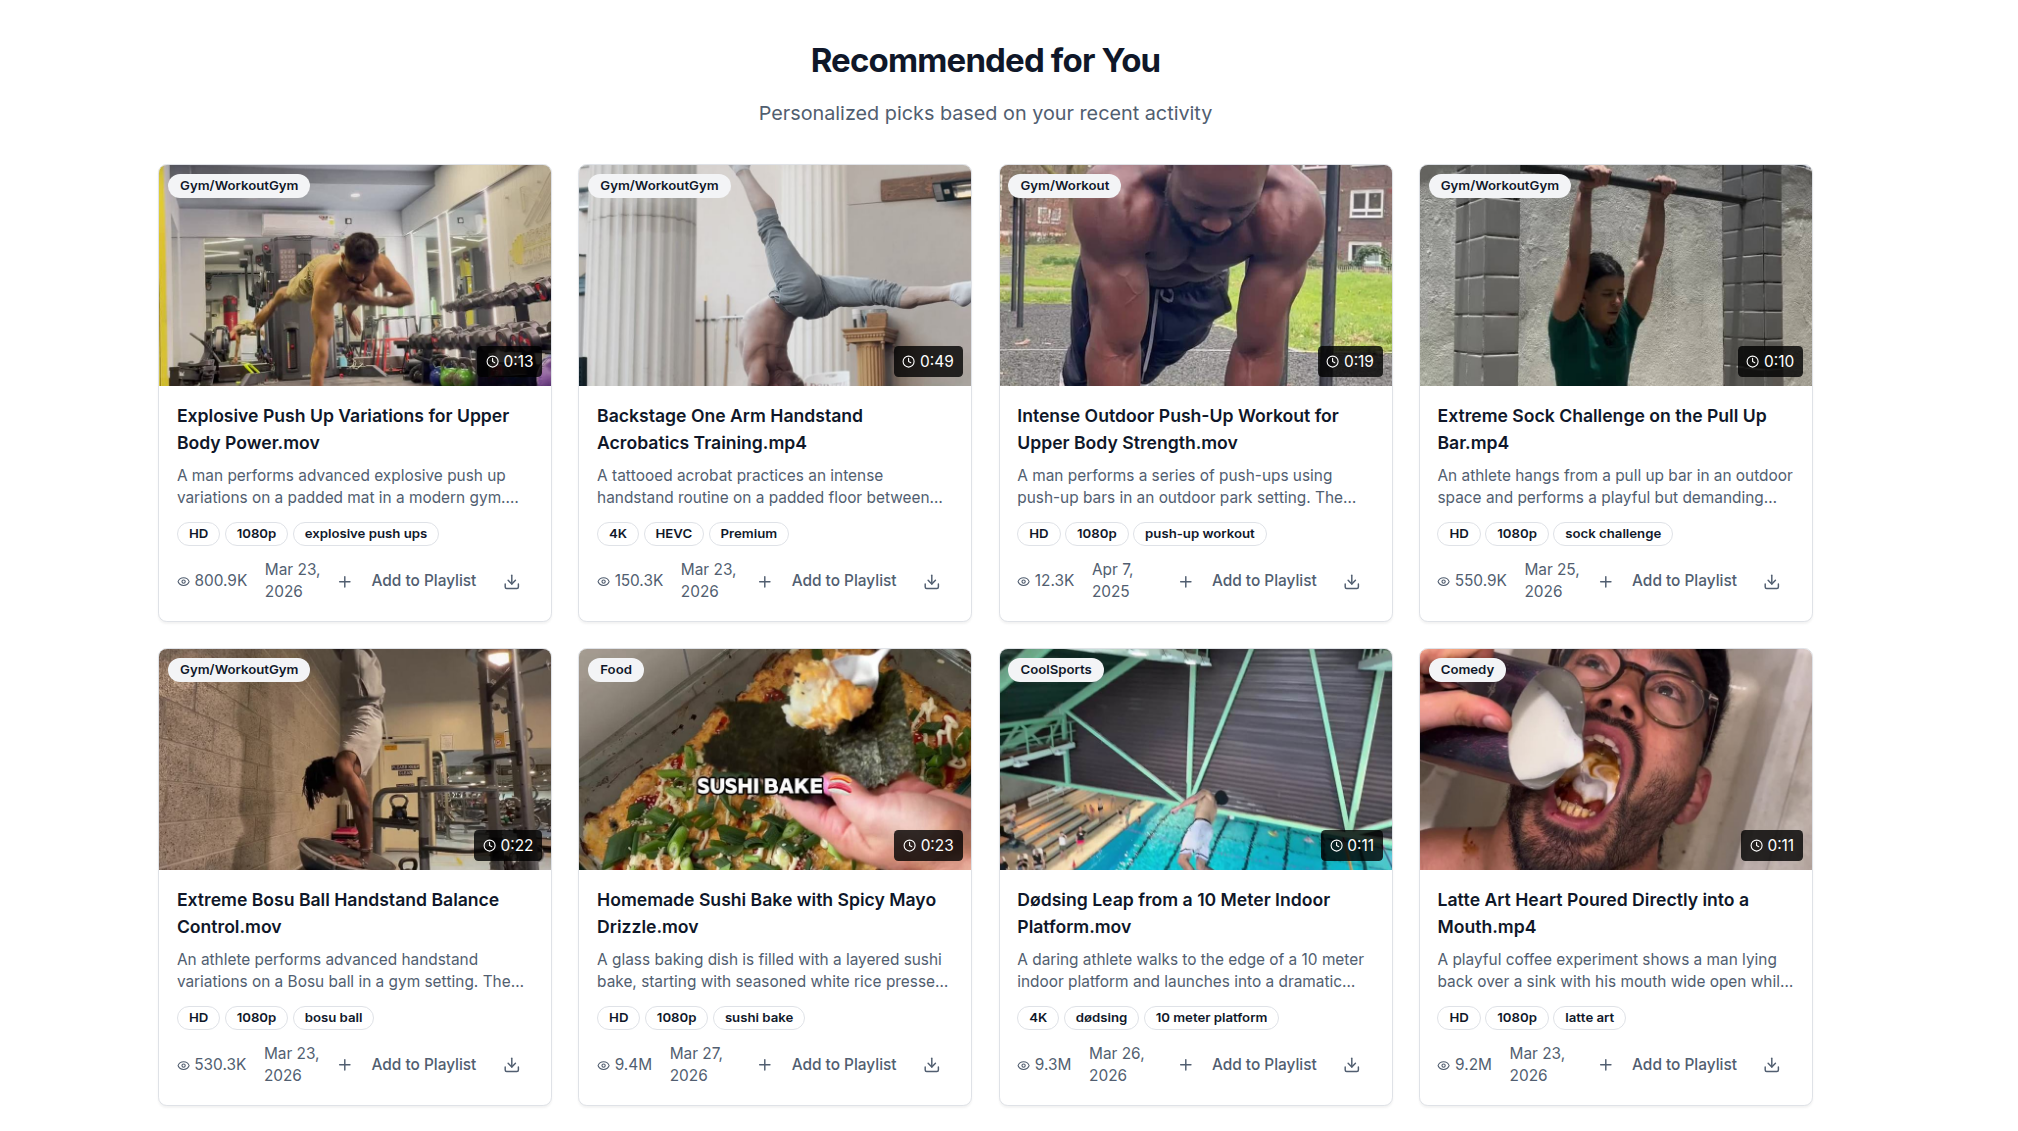
\includegraphics[width=\textwidth]{figures/videosearch/recommended for you page.png}
\caption{``Recommended for You'' section on the Video Search Portal home dashboard}
\label{fig:rec_ui}
\end{figure}

\section*{Conclusion}
\addcontentsline{toc}{section}{Conclusion}

Sprint 5 introduced a \textbf{personalized recommendation engine} driven by real-time
behavioural signals — search queries, click events, and playlist additions. A per-user interest
profile with exponential weight decay captures evolving preferences without requiring scheduled
recomputation jobs. The blended candidate pipeline, combining personalized and trending results
with freshness, diversity, and exploration controls, delivers a feed that improves with every
user interaction. Three new PostgreSQL tables and one Alembic migration extend the AR-API
schema, completing the personalization layer of the BVIRAL platform.
